\section{D. Irga B. Naufal Fakhri}
\subsection{Pemahaman Teori}
\begin{enumerate}
\item Device Manager pada Windows dan folder /dev pada Linux

Device manager adalah system tools yang fungsinya untuk mengidentifikasi dan mengelola hardware serta driver yang diperlukan oleh hardware yang dihubungkan. Device Manager juga bisa mengenali hardware dan menginstall drivernya secara otomatis, tapi kalo driver dari hardware tersebut tidak ada pada koleksi driver Windows, maka Device Manager akan memberikan notifikasi dan tanda khusus bahwa hardware tersebut membutuhkan driver terpisah agar bisa terinstall dengan benar.

/dev pada Linux merupakan direktori yang berfungsi untuk menyimpan konfigurasi device atau hardware dari sistem, seperti harddisk (hda, sda), terminal (tty) dll.

\item Jelaskan langkah-langkah instalasi driver dari arduino

Apabila anda menggunakan Arduino versi original maka drivernya akan diinstall saat anda menginstall Arduino IDE saat anda menhubungkan Arduino anda ke PC menggunakan kabel USB. Jika anda menggunakan Arduino Uno SMD Clone seperti saya maka anda harus menginstall drivernya terlebih dahulu setelah menginstall Arduino Uno, Caranya:
	\begin{itemize}
	\item Buka program setup.exe pada folder DRIVER1
	\begin{figure}[ht!]
		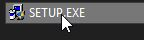
\includegraphics[width=5cm]{figures/5/1174066/0.jpg}
		\centering
		\caption{Setup}
	\end{figure}
	
	\item Setelah itu klik Install
	\begin{figure}[ht!]
		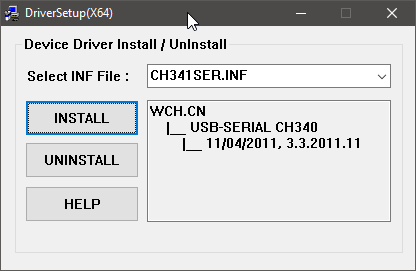
\includegraphics[width=5cm]{figures/5/1174066/1.png}
		\centering
		\caption{Instalasi}
	\end{figure}

	\item Setelah muncul seperti dibawah ini tekan OK
	\begin{figure}[ht!]
		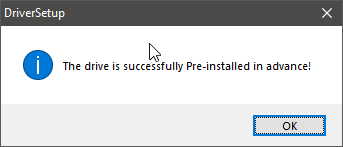
\includegraphics[width=5cm]{figures/5/1174066/2.png}
		\centering
		\caption{Instalasi Berhasil}
	\end{figure}

	\item Hubungkan Arduino ke PC, lalu buka device manager\begin{figure}[ht!]
		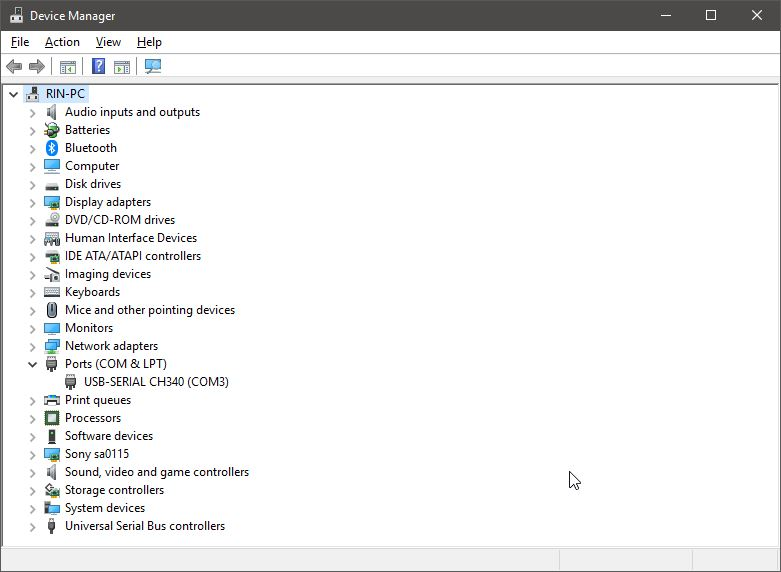
\includegraphics[width=5cm]{figures/5/1174066/3.jpg}
		\centering
		\caption{Device Manager}
	\end{figure}

	\item Lalu pilih pada bagian port apabila seperti ini maka driver arduino telah terinstall\begin{figure}[ht!]
		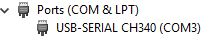
\includegraphics[width=5cm]{figures/5/1174066/4.jpg}
		\centering
		\caption{Arduino Terdeteksi}
	\end{figure}
	
	\end{itemize}

\item Jelaskan bagaimana cara membaca baudrate dan port dari komputer yang sudah terinstall driver

Cara membaca baudrate adalah dengan cara membuka arduino ide lalu mengclik serial monitor yang iconnya seperti kaca pembesar(Cari). 
Untuk mengecek port kita bisa melihatnya melalu device manager pada bagian ports, yang ada tulisan COMXX (XX adalah angka dari COM) itu adalah portnya
	
\item Jelaskan sejarah library pyserial

pySerial adalah modul API Python untuk mengakses port serial. pySerial menyediakan API yang seragam di berbagai sistem operasi, termasuk Windows, Linux, dan BSD.

\item Jelaskan fungsi-fungsi apa saja yang dipakai dari library pyserial

	\begin{itemize}
	\item Serial()
	
	Berfungsi untuk membuka port serial.
	
	\item Write()
	
	Berfungsi untuk mengirimkan data string ke port serial dan mengembalikan nomor bytes yang terkirim.
	
	\item Read(size)
	
	Berfungsi untuk membaca data dari port serial.
	
	\item Readline(size)
	
	Berfungsi untuk membaca line sampai line terakhir (EOL). 
	
	\item Close()
	
	Berfungsi untuk menutup pembacaan port serial.
	\end{itemize}

\item Jelaskan kenapa butuh perulangan dan tidak butuh perulangan dalam membaca serial

Perulangan dalam python berfungsi untuk mengulangi kode/perintah yang ada didalam perulangan tersebut. ada dua macam perulangan pada python, yang pertama for dan yang kedua while.
Perbedaan for dan while adalah for yaitu perulangan yang menghitung (Counted Loop) sedangkan while adalah perulangan yang tidak terhitung (Uncounted Loop). Penggunakan for itu biasanya jika untuk mengulangi kode yang akan ditentukan berapa kali diulangnya sedangkan while digunakan jika ada syarat tertentu untuk mengulangi kode itu dan tidak menentu berapa banyak perulangannya.
Mengapa diperlukan perulangan, karena agar data yang dibaca tidak hanya satu kali saja namun berkali kali, dengan adanya perulangan kita bisa membaca datanya berulang kali. Sehingga data yang kita baca dapat muncul lebih dari satu. Sedangkan kalau kita tidak memakai perulangan maka data yang muncul hanya satu.

\item Jelaskan bagaimana cara membuat fungsi yang mengunakan pyserial

Pembuatan fungsi sama seperti pembuatan fungsi seperti biasanya namun method dari pyserial dimasukkan kedalam fungsi dan dipanggil fungsi yang kita buat tadi
\lstinputlisting[firstline=7, lastline=14]{src/5/1174066/Teori/1174066.py}

\item Scan Plagiarisme
\begin{figure}[ht!]
	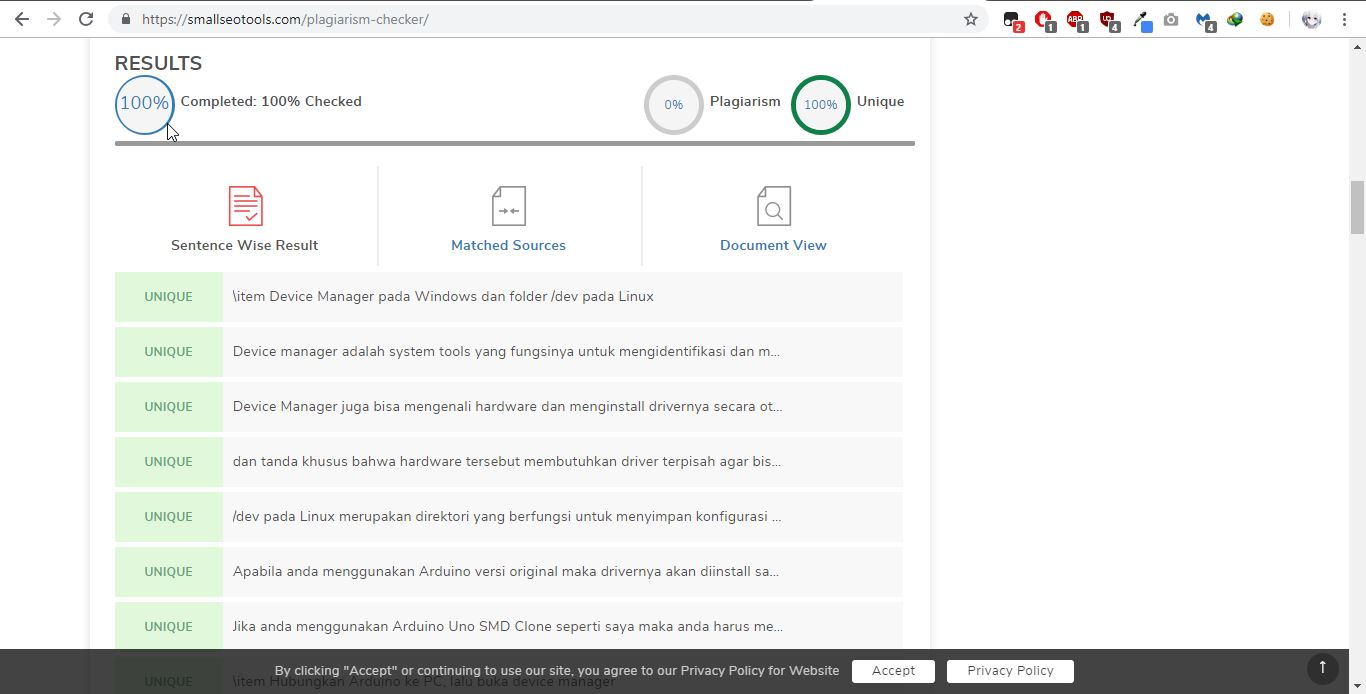
\includegraphics[width=5cm]{figures/5/1174066/plagiat.jpg}
	\centering
	\caption{Plagiarisme}
\end{figure}
\end{enumerate}